\documentclass[aspectratio=1610, xcolor={dvipsnames}]{beamer}

\usetheme[
    % options
]{metropolis}

\setbeamercolor{background canvas}{bg = white}

% macro.tex

\usepackage{graphicx}
\usepackage{amsmath}
\usepackage{multicol}
\usepackage{tabularx}
\usepackage{array}
\newcolumntype{x}[1]{>{\centering\arraybackslash\hspace{0pt}}p{#1}}
% \setlength{\columnseprule}{1pt}
% \def\columnseprulecolor{\color{block body.fg}}
\usepackage{tikz, pgfplots}
\usetikzlibrary{shapes.geometric, shapes, fit, arrows, calc, fit, positioning, chains, arrows.meta, backgrounds, calc}

% subject specific
\usepackage{amsmath, amssymb}

% drawing
\usepackage{pstricks}
\usepackage{tikz, tkz-orm, pgfplots}
\usetikzlibrary{arrows,shapes,backgrounds,decorations.markings}
\usetikzlibrary{matrix,positioning,decorations.pathreplacing,calc,tikzmark}
\pgfplotsset{width=7.5cm,compat=1.16}
\usepgfplotslibrary{fillbetween}

% listings
\usepackage[final]{listings}
% \usepackage{unicode-math}
% \usepackage{xunicode}
% \usepackage{fontspec}
% \setmonofont[
%   Contextuals={Alternate}
% ]{Fira Code}

\definecolor{codegreen}{rgb}{0,0.6,0}
\definecolor{codegray}{rgb}{0.5,0.5,0.5}
\definecolor{codepurple}{rgb}{0.58,0,0.82}
\definecolor{backcolour}{rgb}{1,1,1}

\lstdefinestyle{stolenstyle}{
    backgroundcolor=\color{backcolour},
    commentstyle=\color{codegreen},
    keywordstyle=\color{magenta},
    numberstyle=\tiny\color{codegray},
    stringstyle=\color{codepurple},
    basicstyle=\ttfamily\footnotesize,
    breakatwhitespace=false,
    breaklines=true,
    captionpos=b,
    keepspaces=true,
    numbers=left,
    numbersep=5pt,
    showspaces=false,
    showstringspaces=false,
    showtabs=false,
    tabsize=2,
    inputencoding=utf8,
    extendedchars=true,
    language=scala,
    % texcl=false,
    mathescape=false,
    % escapechar=\&,
    literate = 
        {=>}{{=>}} {2}
        {->}{{->}} {2}
        {_}{{\_}} {1}
        {|}{\textbar} {1}
        {==>}{{==>}} {3},
}

\lstset{style=stolenstyle}

\lstdefinestyle{lisa}{
    backgroundcolor=\color{backcolour},   
    commentstyle=\color{codegreen},
    keywordstyle=\color{magenta},
    numberstyle=\tiny\color{codegray},
    stringstyle=\color{codepurple},
    basicstyle=\linespread{1.4}\ttfamily\footnotesize,
    breakatwhitespace=false,         
    breaklines=false,                 
    captionpos=b,                    
    keepspaces=true,                 
    numbers=left,                    
    numbersep=5pt,                  
    showspaces=false,                
    showstringspaces=false,
    showtabs=false,                  
    tabsize=2,
    keywordstyle = [2]{\color{OliveGreen}},
    keywordstyle = [3]{\color{Blue}},
    keywordstyle = [4]{\color{BrickRed}},
    morekeywords = [2]{val, Theorem, have, thenHave, andThen, by},
    morekeywords = [3]{AccOutNil},
    morekeywords = [4]{Apply},
    literate = 
        {===}{{===}} 3
        {::}{{::}}   2
        {->}{{->}}   2,
}

% \lstset{style=lisa}

% links and citations
\usepackage{hyperref, bookmark}
\hypersetup{hidelinks} % hide boxes around links ew
% pls add color
\usepackage{csquotes}
% \usepackage{polyglossia}
% \setdefaultlanguage{english}
\usepackage[
    style=numeric,
    sorting=none,
    maxnames=99,
    language=english
]{biblatex}
\addbibresource{biblio.bib}

\usepackage{mathpartir}
\usepackage{stmaryrd}

\newcommand{\mathcomment}[1]{\text{\textcolor{black!50}{\emph{#1}}}}


\title{Close Encounters of the JMM Kind}
\author{Aleksey Shipilev}

\begin{document}

\begin{frame}
    % hello
    \centering
    {\Large Close Encounters of the Java Memory Model Kind} \\
    {\large Aleksey Shipilev}\\ \vspace{3em}
    Presented by Sankalp Gambhir for the LAMP PL Seminar, 14 Nov 2023
\end{frame}

% thanks
\begin{frame}
    \frametitle{This is a summary of a long-running discussion}

    Thanks to:

    \begin{itemize}
        \item Simon Guilloud, Shardul Chiplunkar, Matt Bovel, Viktor Kun\v cak, other CS 206 teaching staff
        \item Guillaume Martres and S\'ebastien Doeraene for answering stupid questions
        \item Guillaume specially for the references for this talk!
    \end{itemize}
    

\end{frame}

% what is a memory model
\begin{frame}
    \frametitle{What is a memory model?}

    \begin{itemize}[<+->]
        \item Spec describes an abstract machine model
        \item The model has to subsume memory interactions
        \item This description is the memory model
        \item Can be largely disconnected from the rest of the model
        \item But forms its foundations
    \end{itemize}

\end{frame}

% sequential

\begin{frame}[fragile]
    \frametitle{Sequential Code}

    \begin{lstlisting}
                // main thread
                var x: Int = 0
                val a0 = x
                x = 1
                val a1 = x
                x = 2
                val a2 = x
                x = 3
                val a3 = x
                x = 4
                val a4 = x
                x = 5
                val a5 = x
                (a0, a1, a2, a3, a4, a5)
                // (0, 1, 2, 3, 4, 5)
    \end{lstlisting}

\end{frame}

% SC
\begin{frame}[fragile]
    \frametitle{Sequential Consistency}

    \begin{multicols}{3}
\begin{lstlisting}
// t0
x = 1
y = 1
println(x)
\end{lstlisting}
\columnbreak
\begin{lstlisting}
// t1
x = 2
println(y)
y = 2
println(x)
\end{lstlisting}
\columnbreak

\pause
The result should be an interleaving of the events
    \end{multicols}

    \pause
    As the name suggests, as close to emulating sequential behaviour as
    possible. \pause Standard mental model of programmers too.

\end{frame}

% non SC behaviour

\begin{frame}[fragile]
    \frametitle{Running a small test}

    \centering
    \begin{lstlisting}
var a: Boolean = false
var b: Boolean = false
    \end{lstlisting}

    \begin{multicols}{2}

        \begin{lstlisting}
// t0
a = true
if b then
  0
else 
  1
        \end{lstlisting}

        \columnbreak

        \begin{lstlisting}
// t1
b = true
if a then
  0
else 
  1
        \end{lstlisting}
        
    \end{multicols}

    Outputs? \\ \pause
    (0, 0)? \pause
    (1, 0)? \pause
    (0, 1)? \pause
    (1, 1)?
    

\end{frame}

\begin{frame}[fragile]
    \frametitle{Running a small test}

    \begin{multicols}{2}
        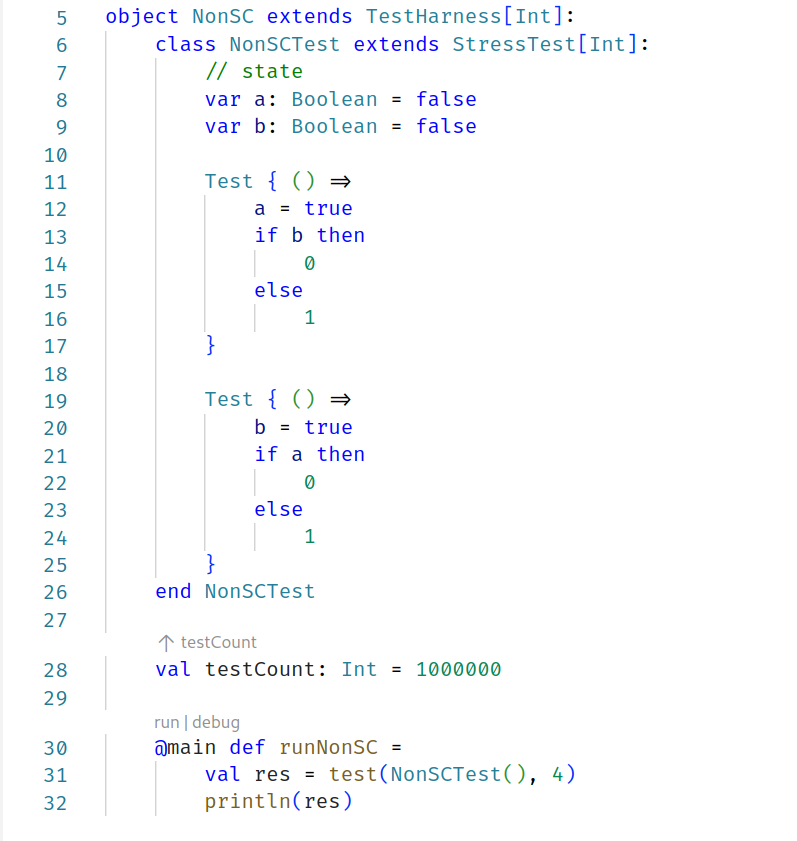
\includegraphics[width=\columnwidth]{fig/nonsctest.png} 

        \columnbreak

        \pause
        \vfill
        \begin{lstlisting}[numbers=none]
Map(
    List(1, 0) -> 499854, 
    List(0, 1) -> 500141, 
    List(0, 0) -> 1, 
    List(1, 1) -> 4
)
        \end{lstlisting}

        \pause

        \centering
        Only \(\sim 0.0004\%\) cases! 
    \end{multicols}

\end{frame}

\begin{frame}
    
    \begin{quote}
        It ain't what you don't know that gets you into trouble. It's what you
        know for sure that just ain't so. 
    \end{quote}

    \hfill - \emph{Mark Twain}

\end{frame}

% JMM quote
\begin{frame}
    \frametitle{Just read the spec!}

    \centering
    \begin{quote}
        The Java Memory Model is the most complicated part of Java spec that must be
        understood by at least library and runtime developers. Unfortunately, it is
        worded in such a way that it takes a few senior guys to decipher it for each
        other. Most developers, of course, are not using JMM rules as stated, and
        instead make a few constructions out of its rules, or worse, blindly copy the
        constructions from senior developers without understanding the limits of their
        applicability. \cite{pragmatics}
    \end{quote}
    
\end{frame}

% rough JMM explanation

% what does the jmm include

\begin{frame}
    \frametitle{Java Memory Model (compacted garbage summary)}

    \begin{itemize}[<+->]
        \item All hail happens-before (hb)
        \item Respect each thread's ordering --- program order (po)
        \item Respect reads and writes --- reads-from (rf)
        \item Synchronization order (so) (the big one)
        \begin{itemize}
            \item volatile ordering (vl)
            \item synchronizes-with (sw/so)
            \item thread ordering (th)
        \end{itemize}
    \end{itemize}

    \pause
    Two conditions for a valid execution:
    \begin{itemize}
        \item no cycles
        \item no invalid reads
    \end{itemize}

\end{frame}

\begin{frame}

    \begin{multicols}{2}
        
        \centering

        \scalebox{1.6}{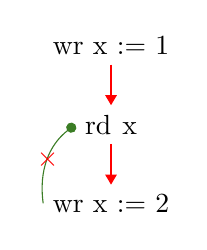
\begin{tikzpicture}
            \node (wr1) {\lstinline|wr x := 1|};
            \node[below of = wr1] (rd) {\lstinline|rd x|};
            \node[below of = rd] (wr2) {\lstinline|wr x := 2|};

            \draw[-Triangle, draw=red] (wr1) -- (rd);
            \draw[-Triangle, draw=red] (rd) -- (wr2);

            \draw[-Circle, draw=OliveGreen, bend left] (wr2.west) to node[midway] {\textcolor{red}{\(\times\)}} (rd.west);
        \end{tikzpicture}}

        \scalebox{1.6}{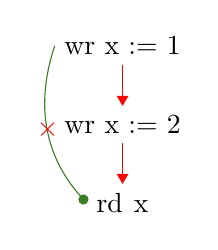
\begin{tikzpicture}
            \node (wr1) {\lstinline|wr x := 1|};
            \node[below of = wr1] (wr2) {\lstinline|wr x := 2|};
            \node[below of = wr2] (rd) {\lstinline|rd x|};

            \draw[-Triangle, draw=red] (wr1) -- (wr2);
            \draw[-Triangle, draw=red] (wr2) -- (rd);

            \draw[-Circle, draw=OliveGreen, bend right] (wr1.west) to node[midway] {\textcolor{red}{\(\times\)}} (rd.west);
        \end{tikzpicture}}

        \columnbreak

    \end{multicols}

\end{frame}

% explaining the behaviour we saw

\begin{frame}
    \frametitle{Explaining the example}

    \centering

    \begin{multicols}{2}
        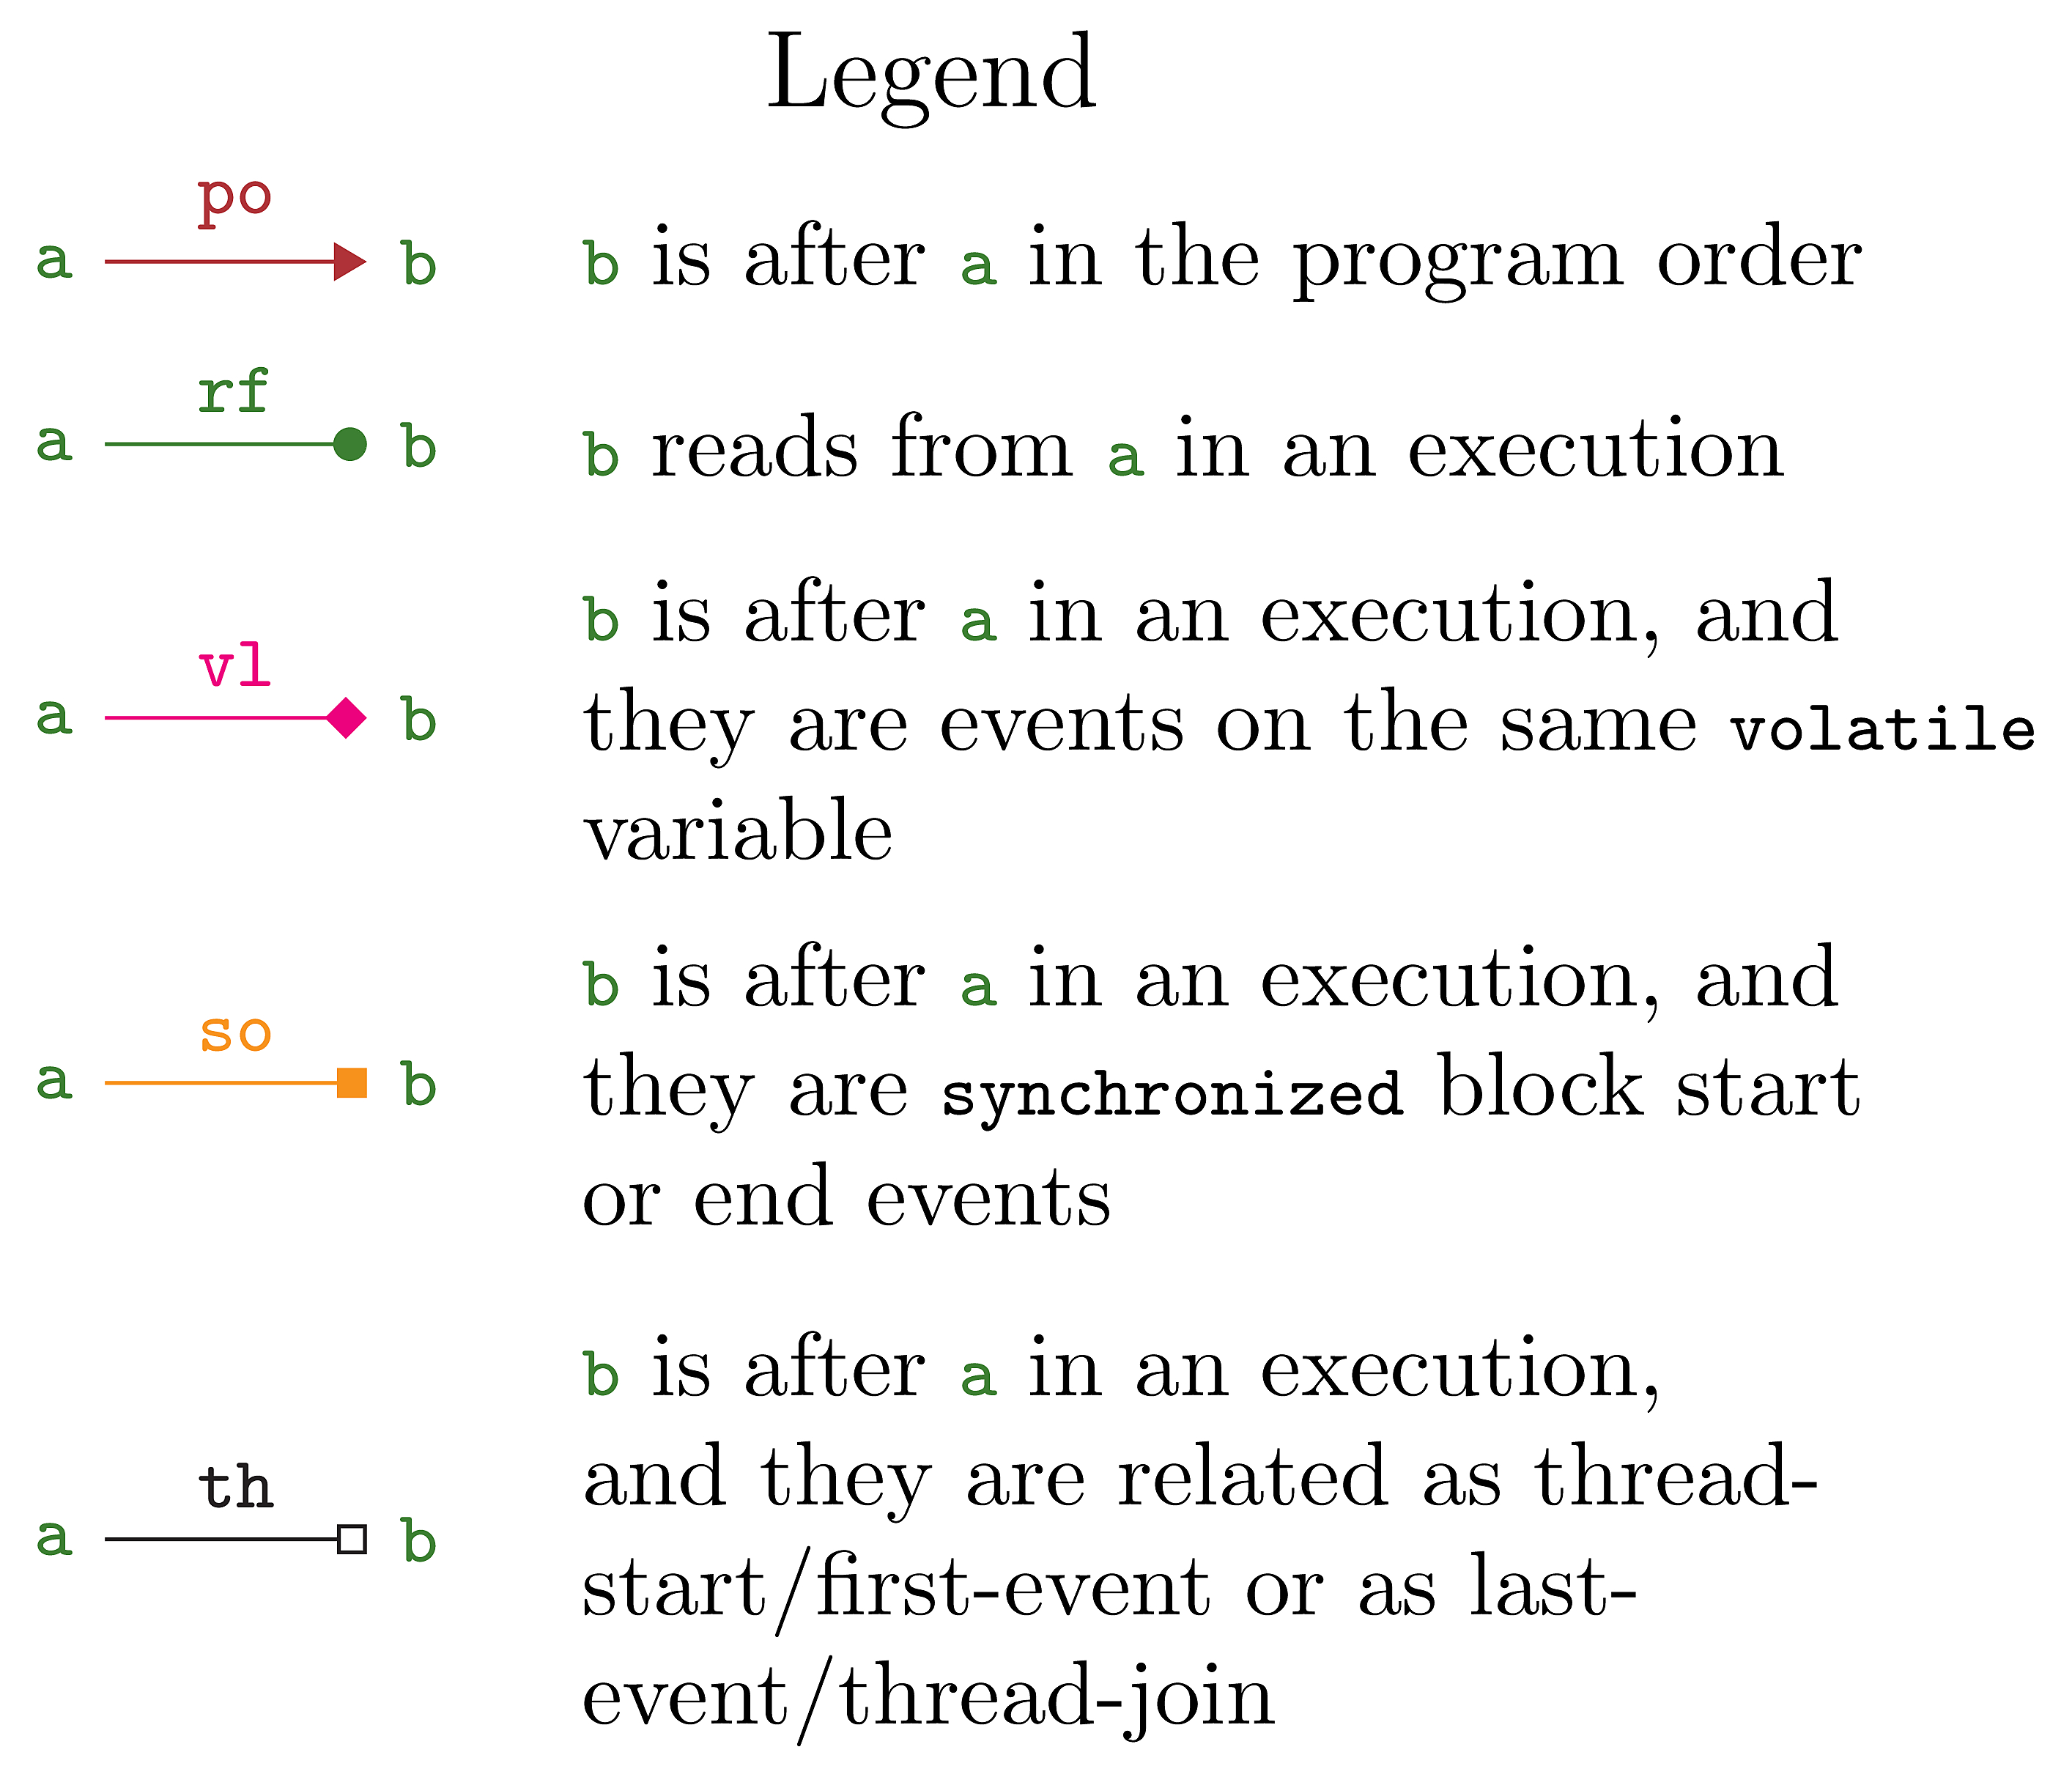
\includegraphics[width=0.45\textwidth]{fig/legend.jpg}
        
        \columnbreak
    
        
\includegraphics[height=10em]{fig/ex_qr.png} \\

        \url{https://lampepfl.github.io/courses/cs206/ex-08-solution-9475bbf99cf472ec48e4} \\ \vspace{2em}
        \url{https://lampepfl.github.io/courses/cs206/ex-08}
    \end{multicols}

\end{frame}

\begin{frame}[fragile]

    \centering
    \begin{lstlisting}
var a: Boolean = false
var b: Boolean = false
var x: Int = -1
var y: Int = -1
    \end{lstlisting}

    \begin{multicols}{2}

        \begin{lstlisting}
// t0
a = true
if b then
  x = 0
else 
  x = 1
        \end{lstlisting}

        \columnbreak

        \begin{lstlisting}
// t1
b = true
if a then
  y = 0
else 
  y = 1
        \end{lstlisting}
        
    \end{multicols}

\end{frame}

\begin{frame}
    \centering
    
    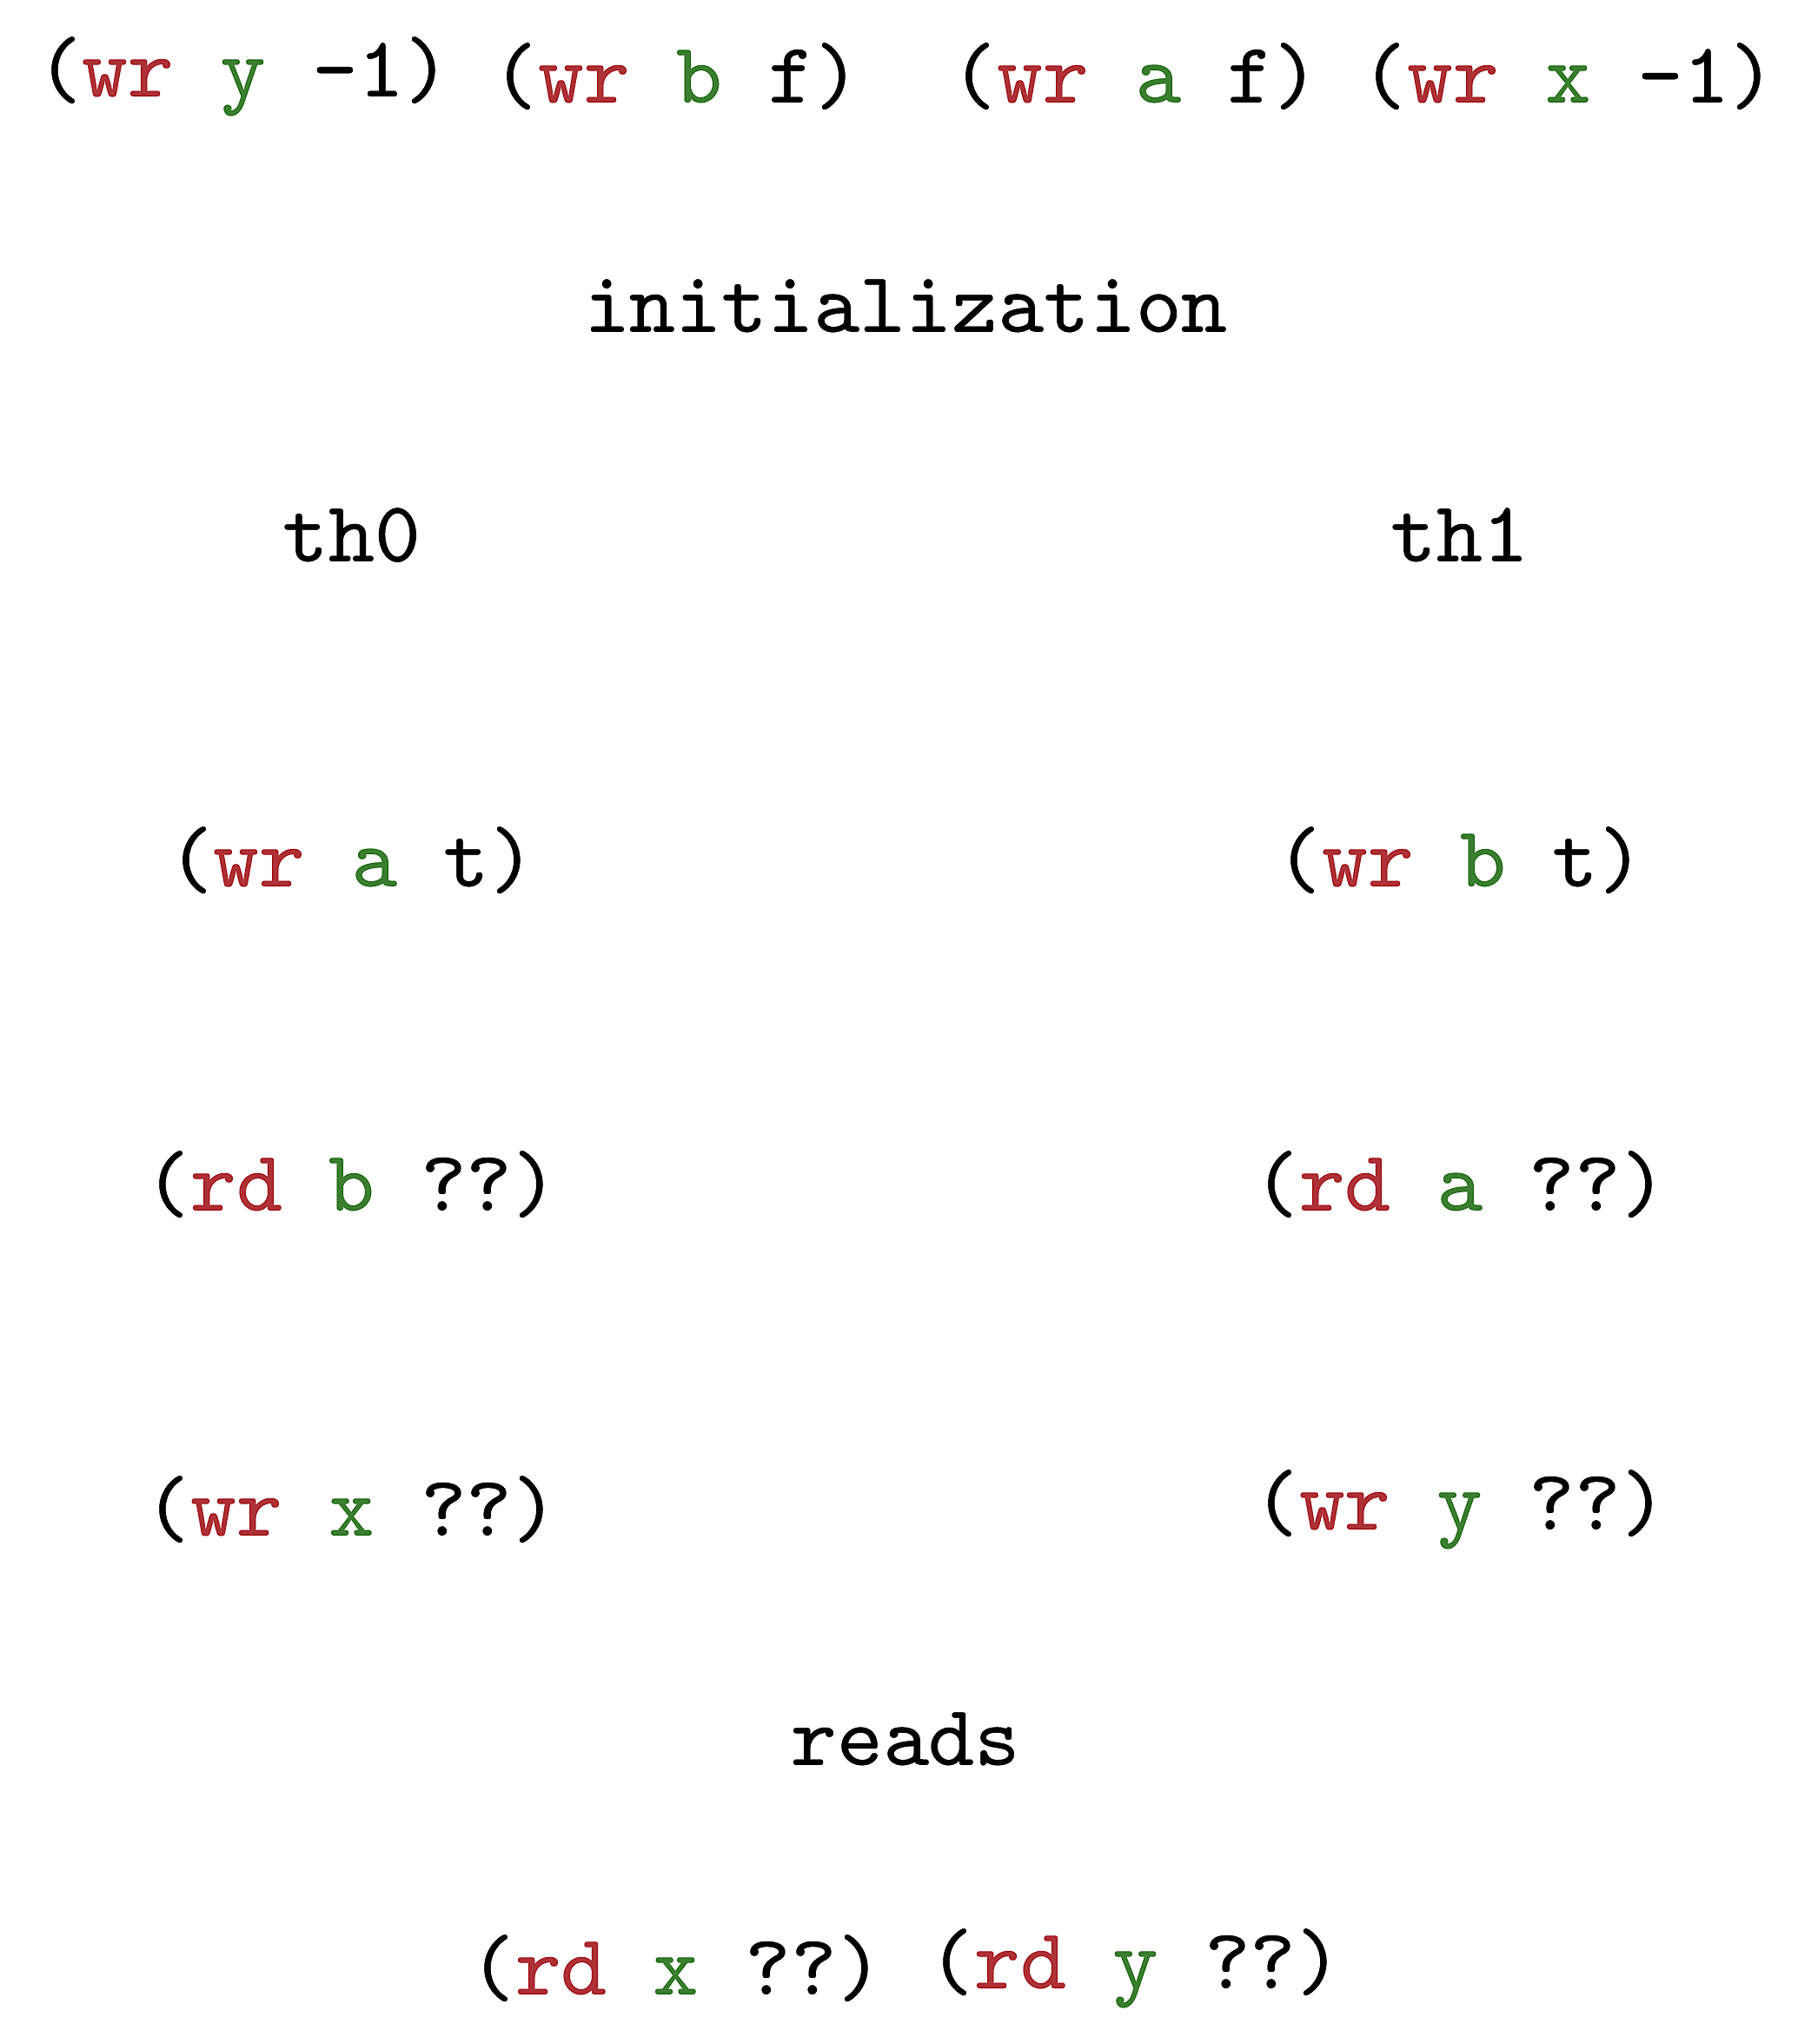
\includegraphics[height=0.9\textheight]{fig/trace5-11-0.jpg}

\end{frame}

\begin{frame}
    \centering
    
    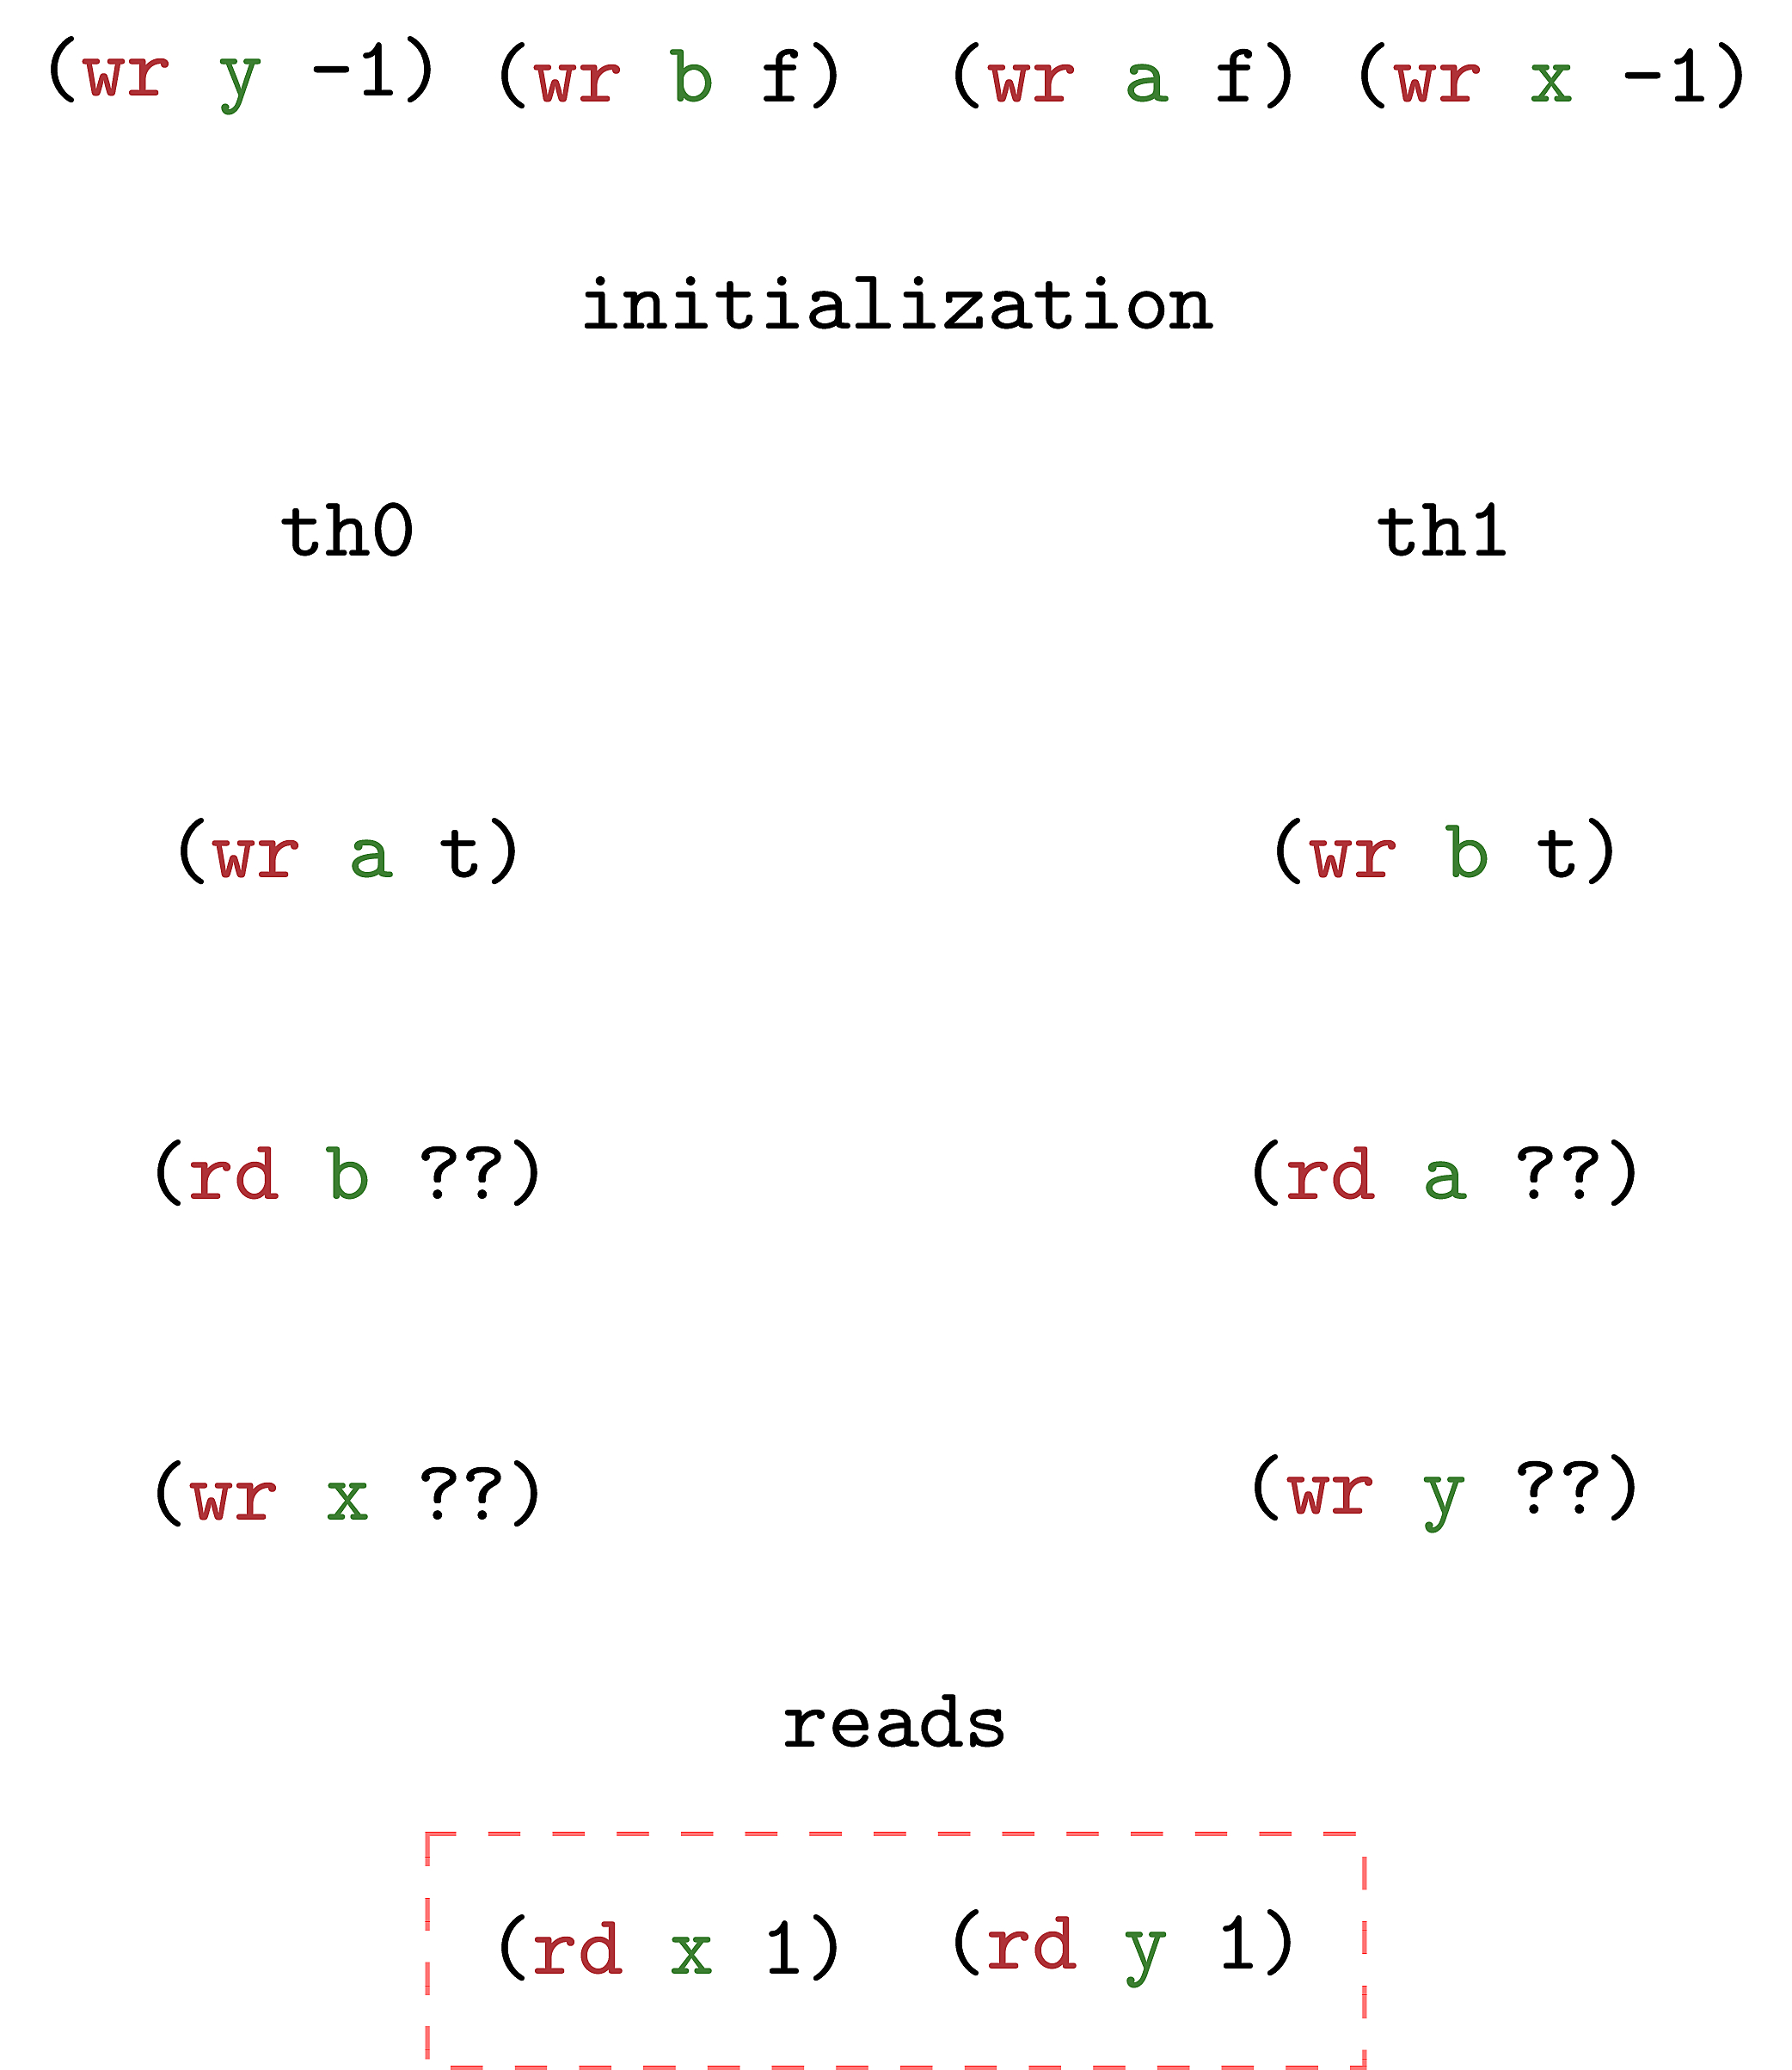
\includegraphics[height=0.9\textheight]{fig/trace5-11-1.jpg}

\end{frame}

\begin{frame}
    \centering
    
    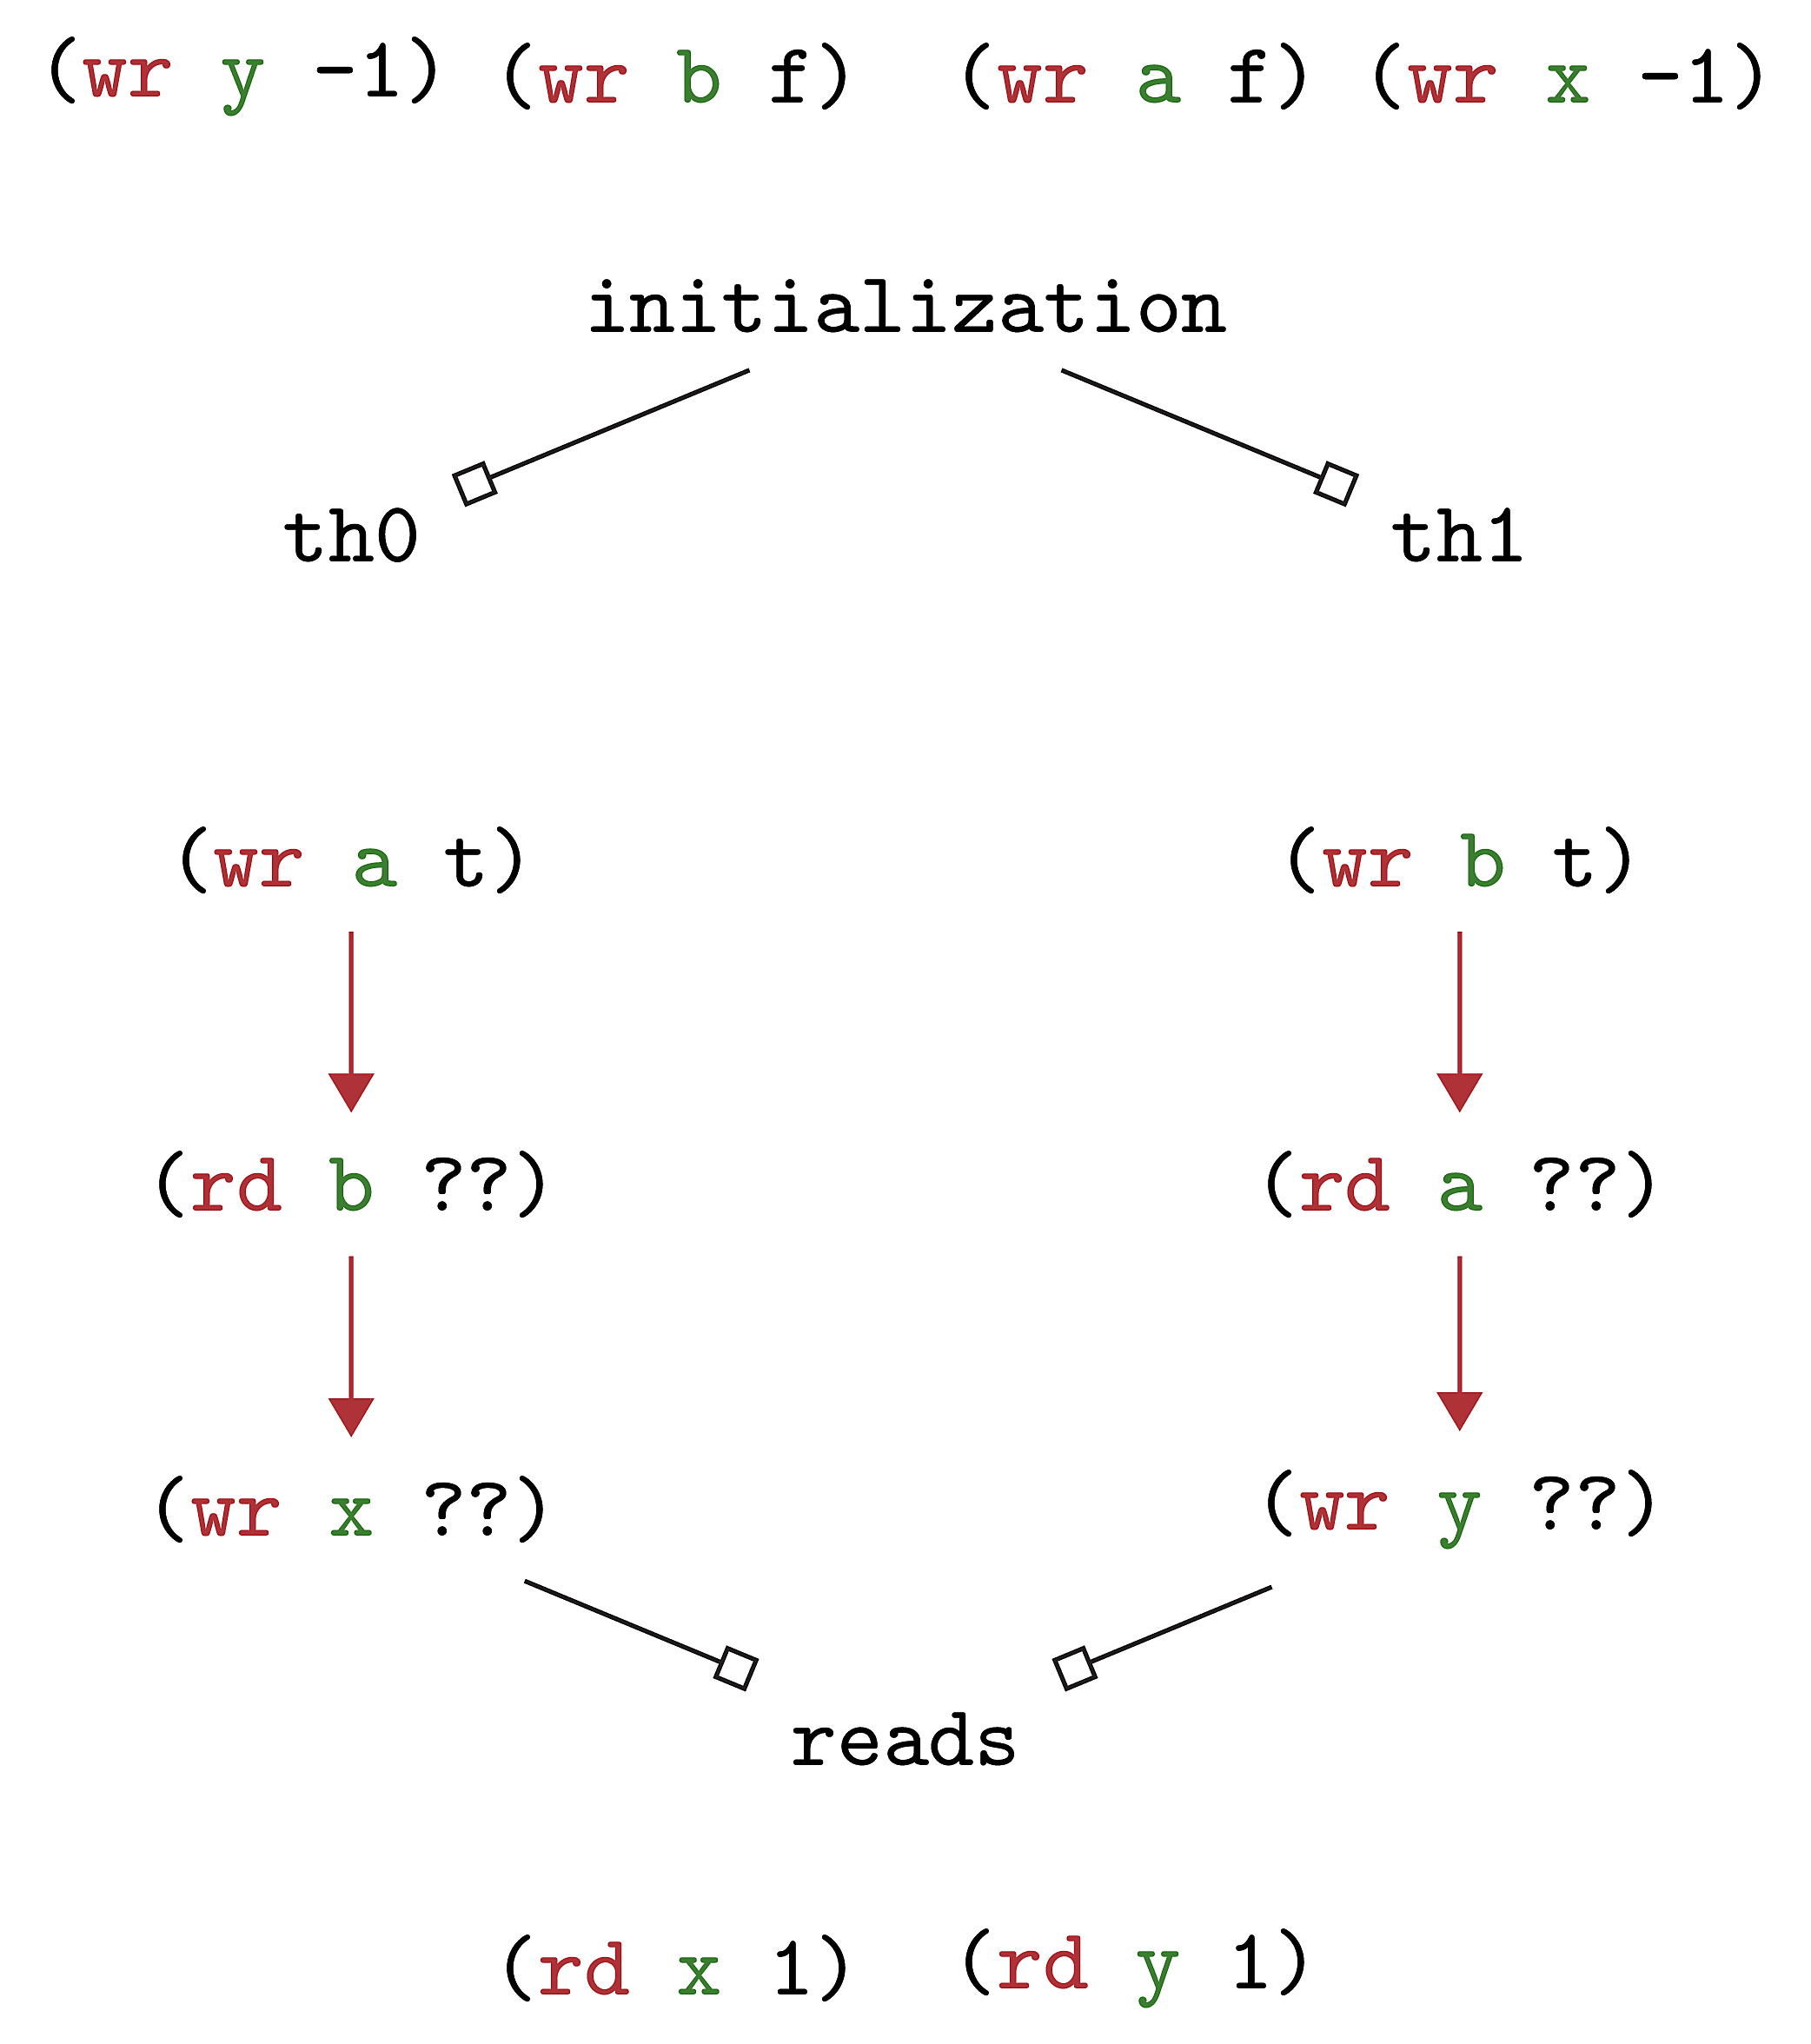
\includegraphics[height=0.9\textheight]{fig/trace5-11-2.jpg}

\end{frame}

\begin{frame}
    \centering
    
    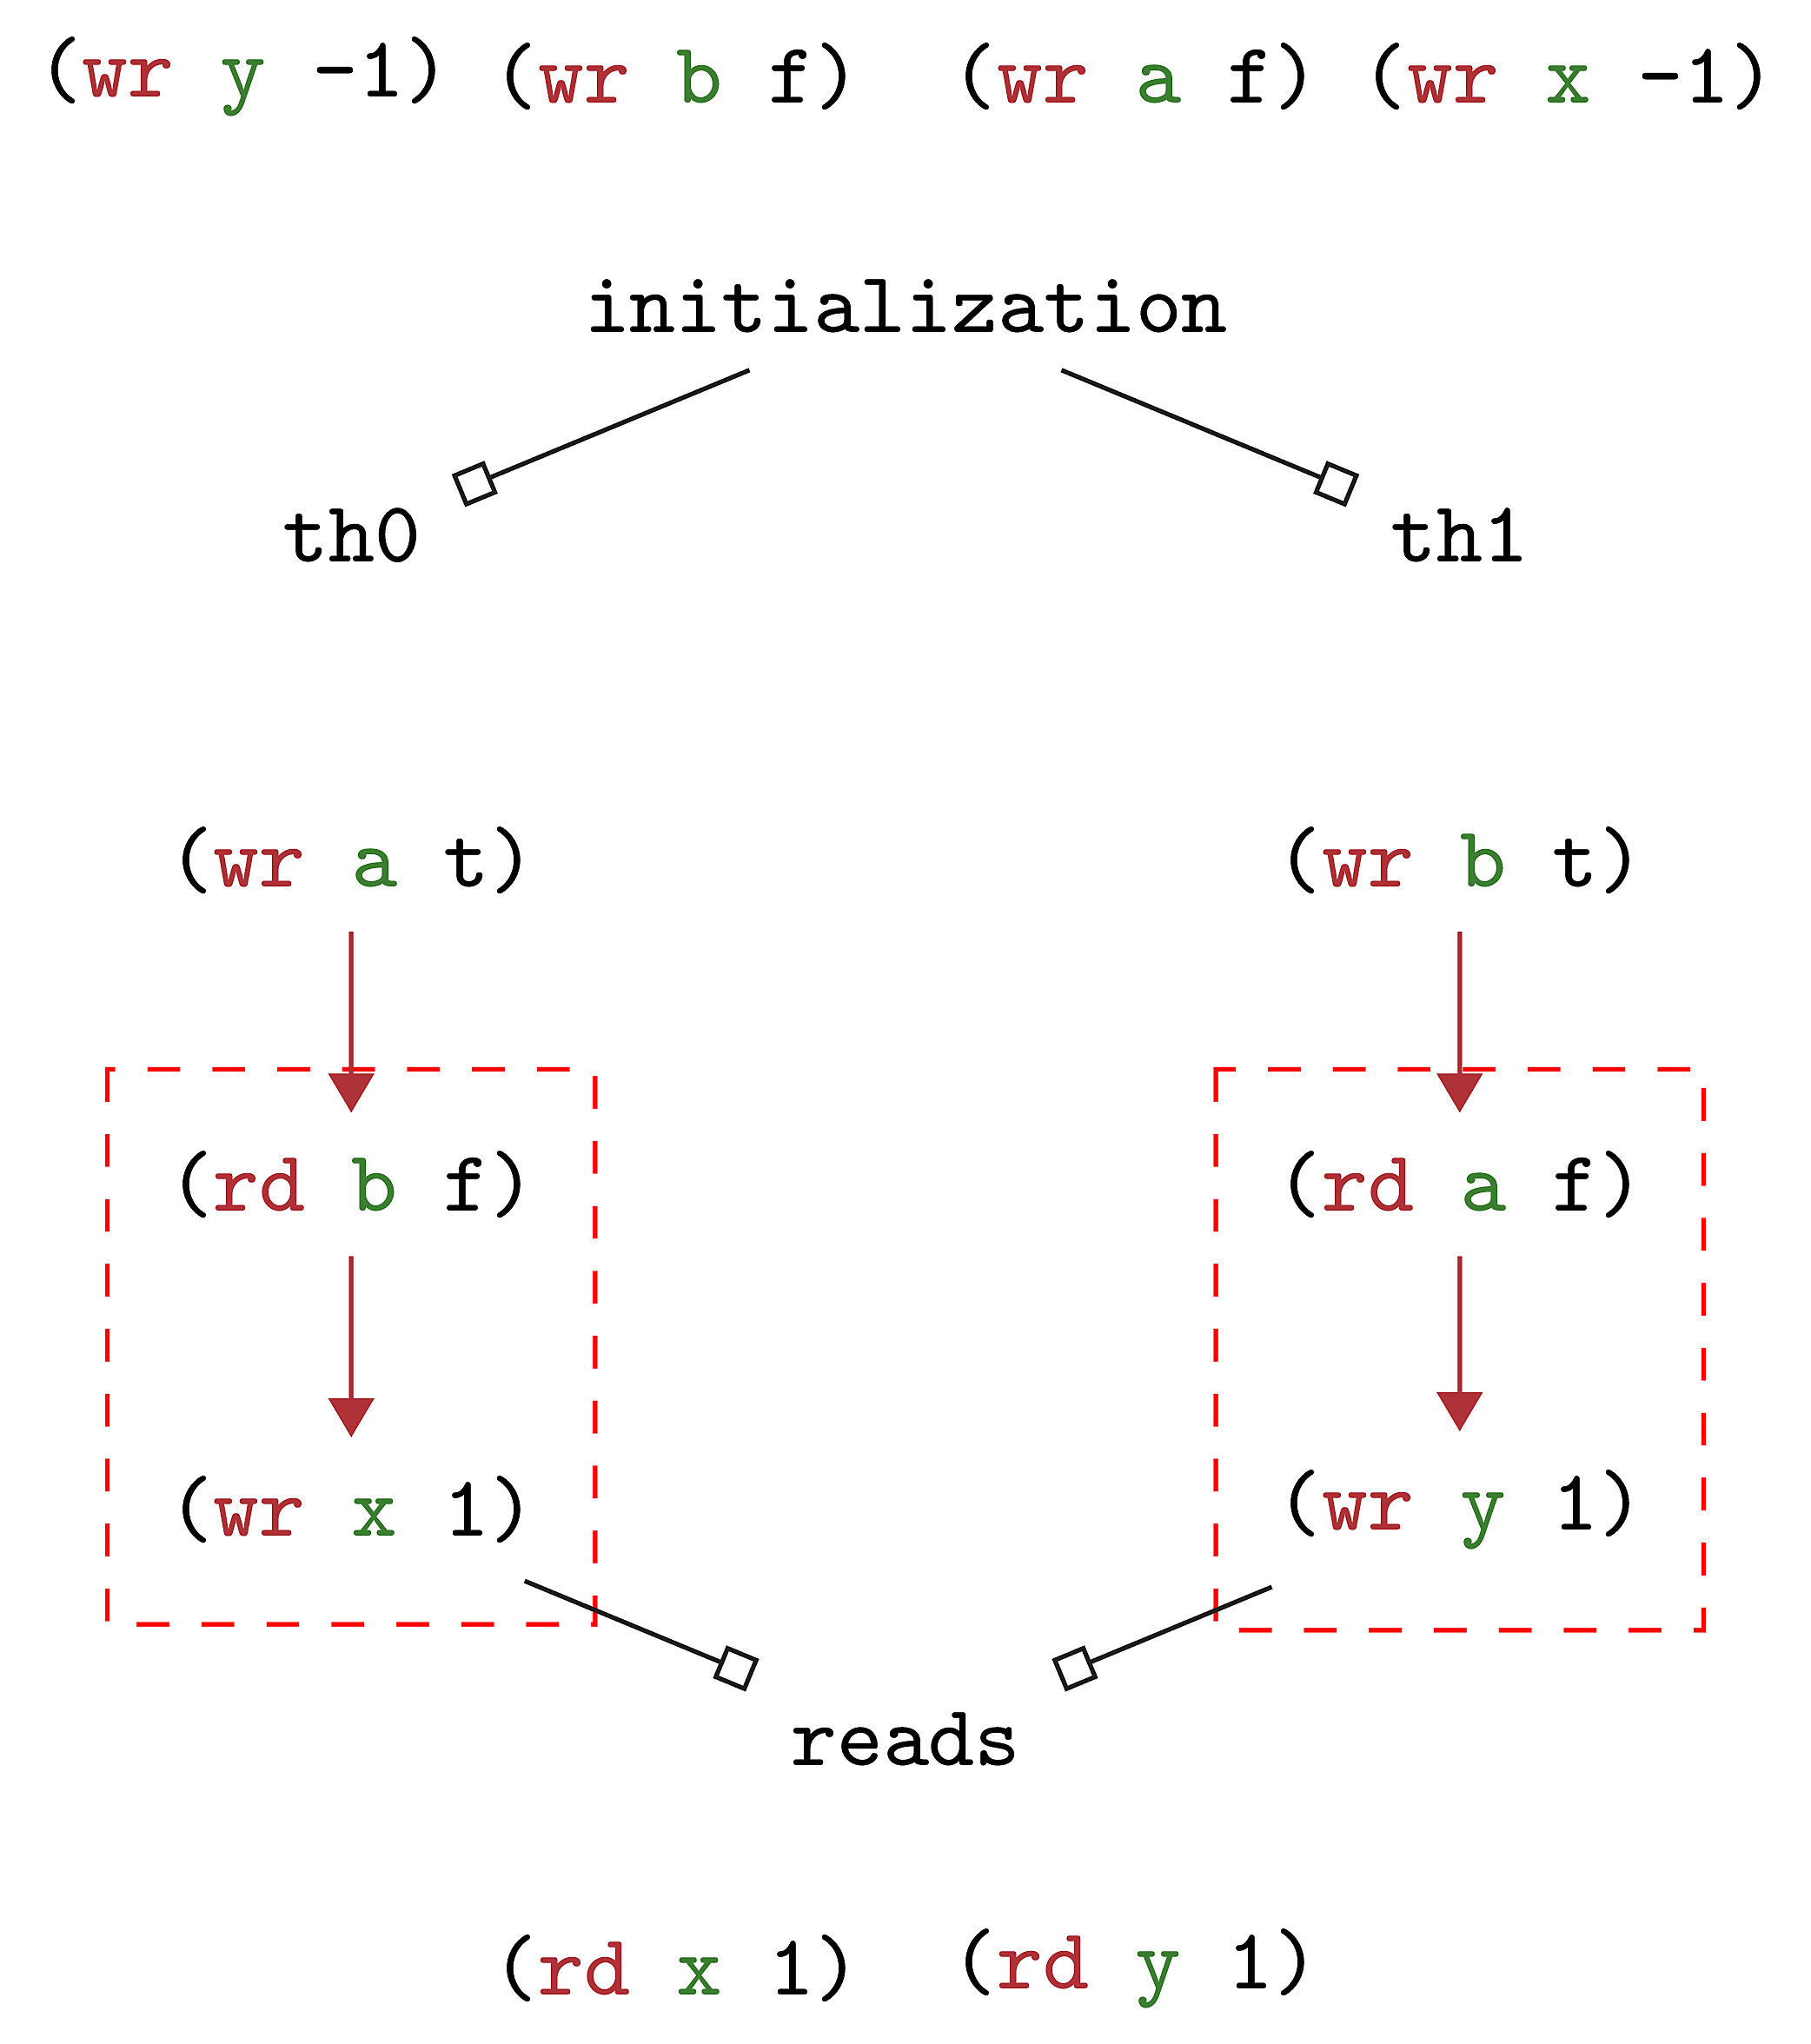
\includegraphics[height=0.9\textheight]{fig/trace5-11-3.jpg}

\end{frame}

\begin{frame}
    \centering
    
    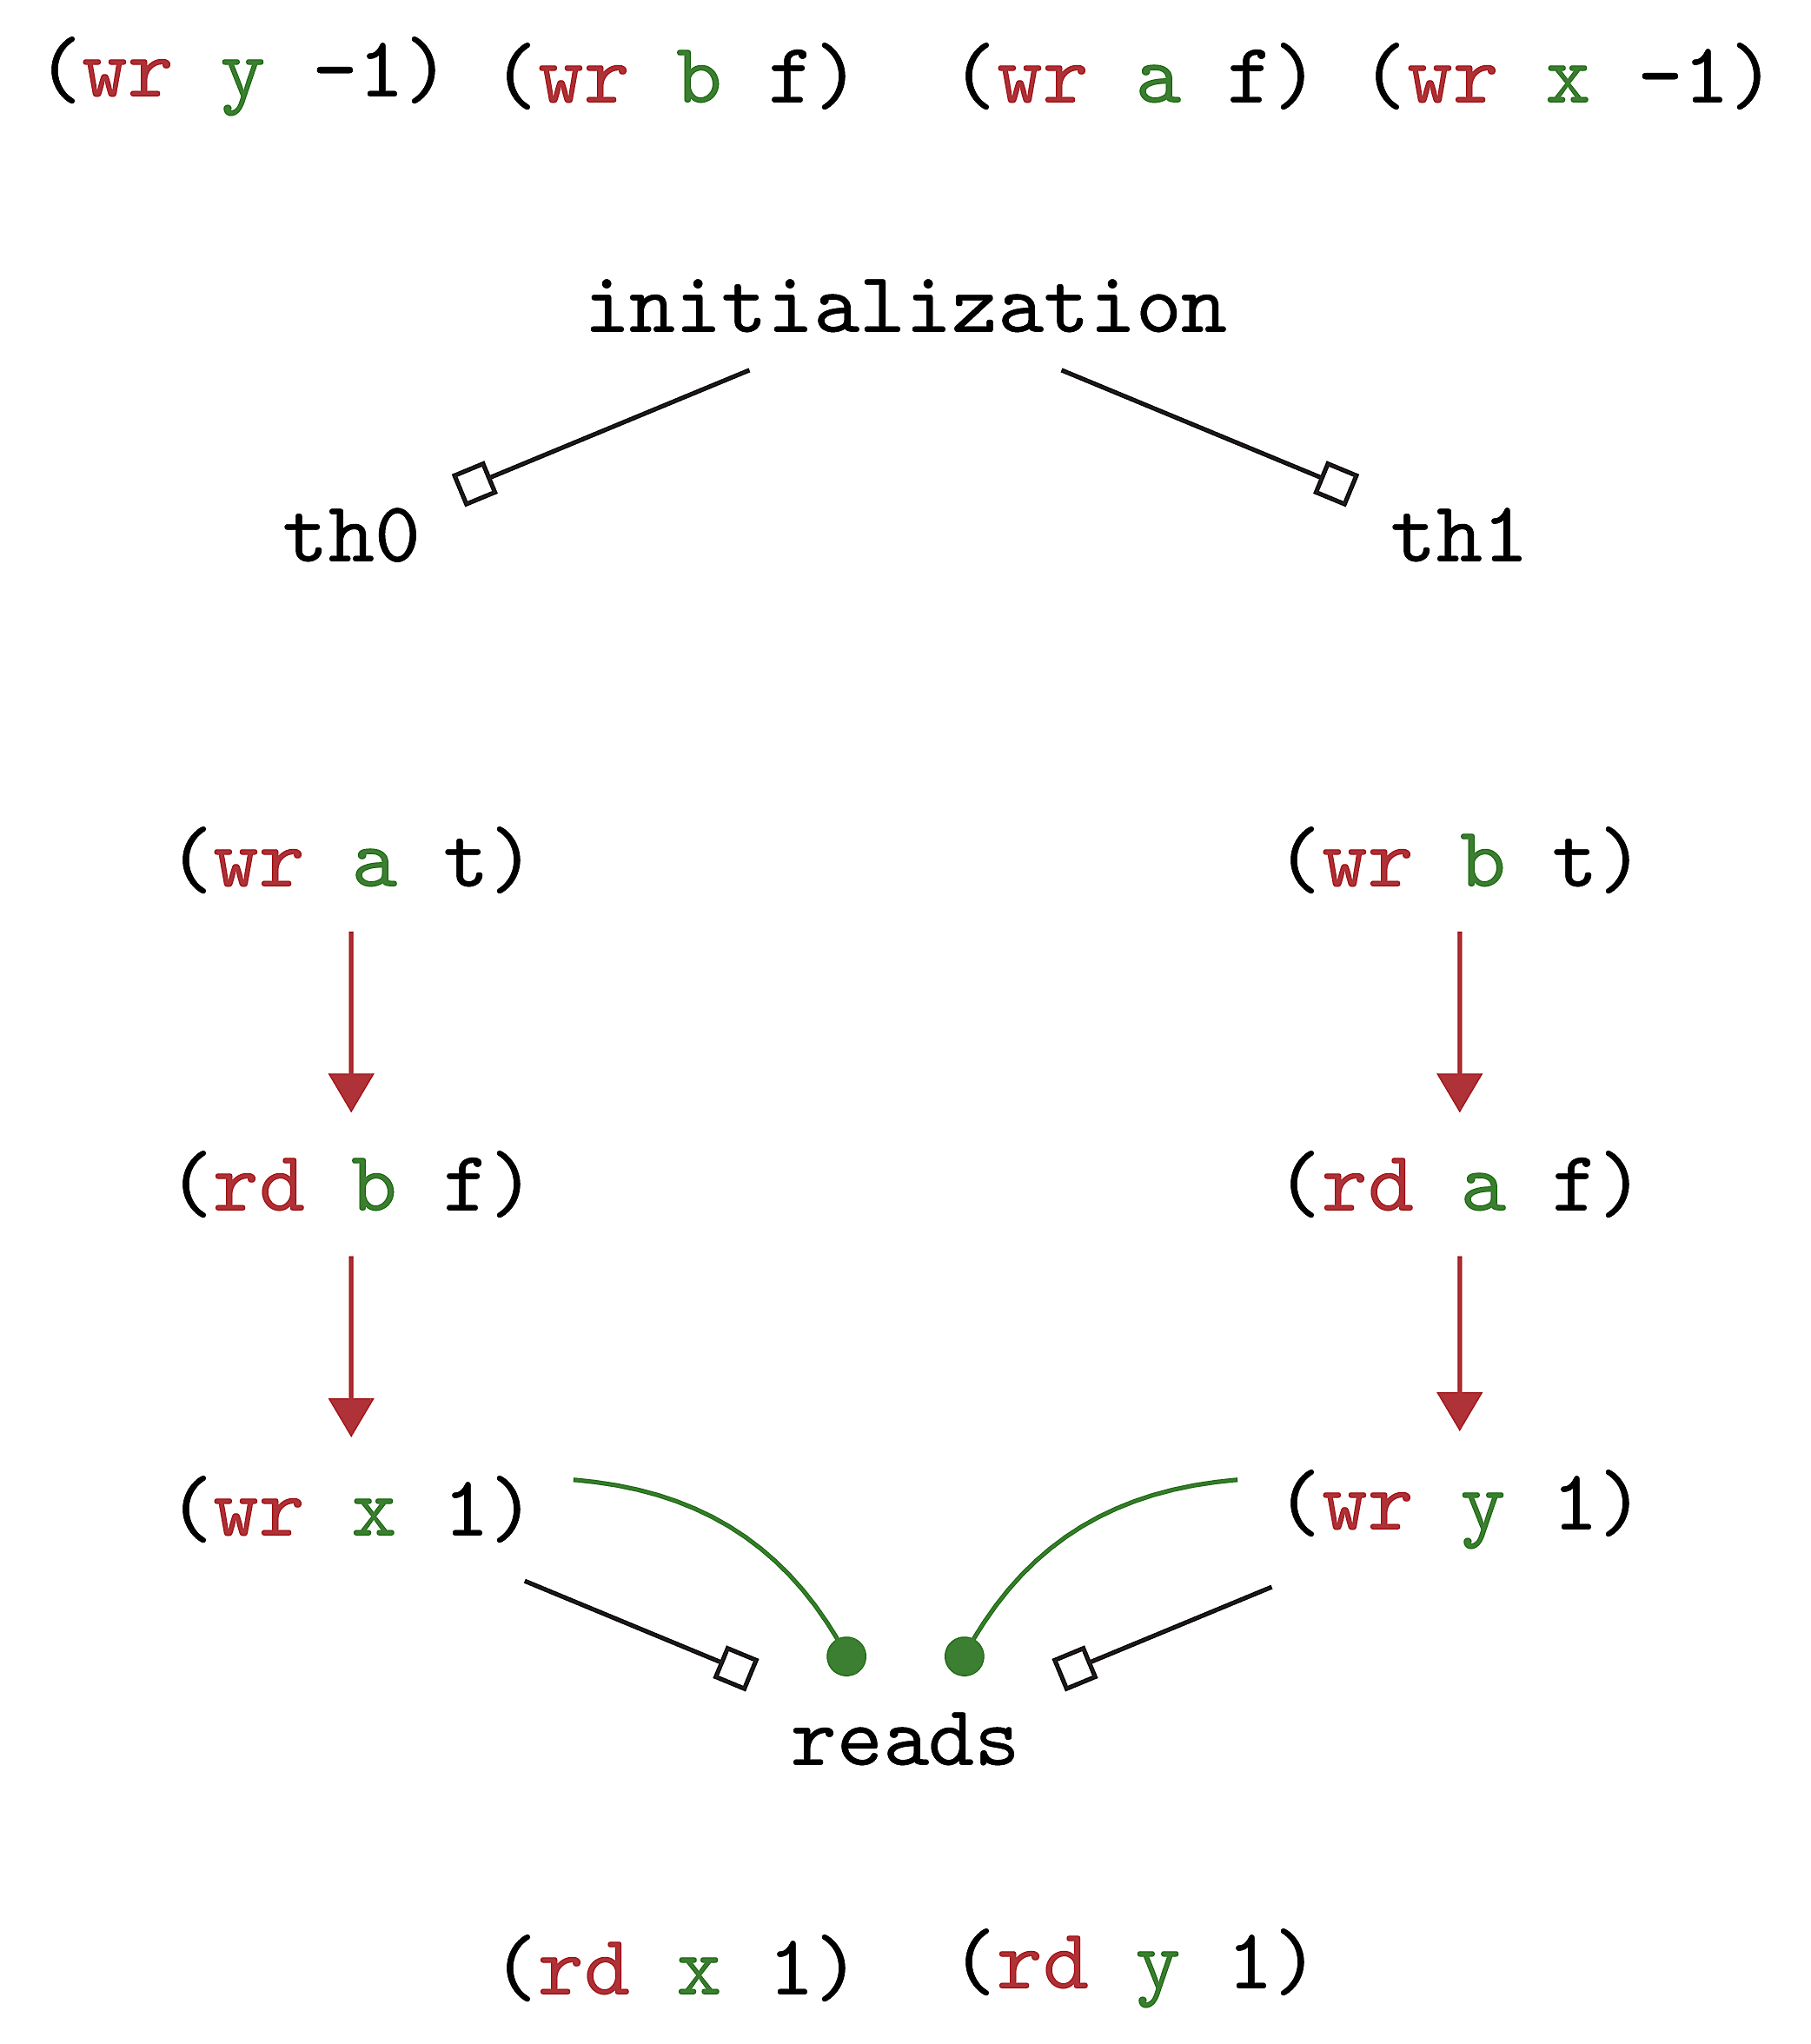
\includegraphics[height=0.9\textheight]{fig/trace5-11-4.jpg}

\end{frame}

\begin{frame}
    \centering
    
    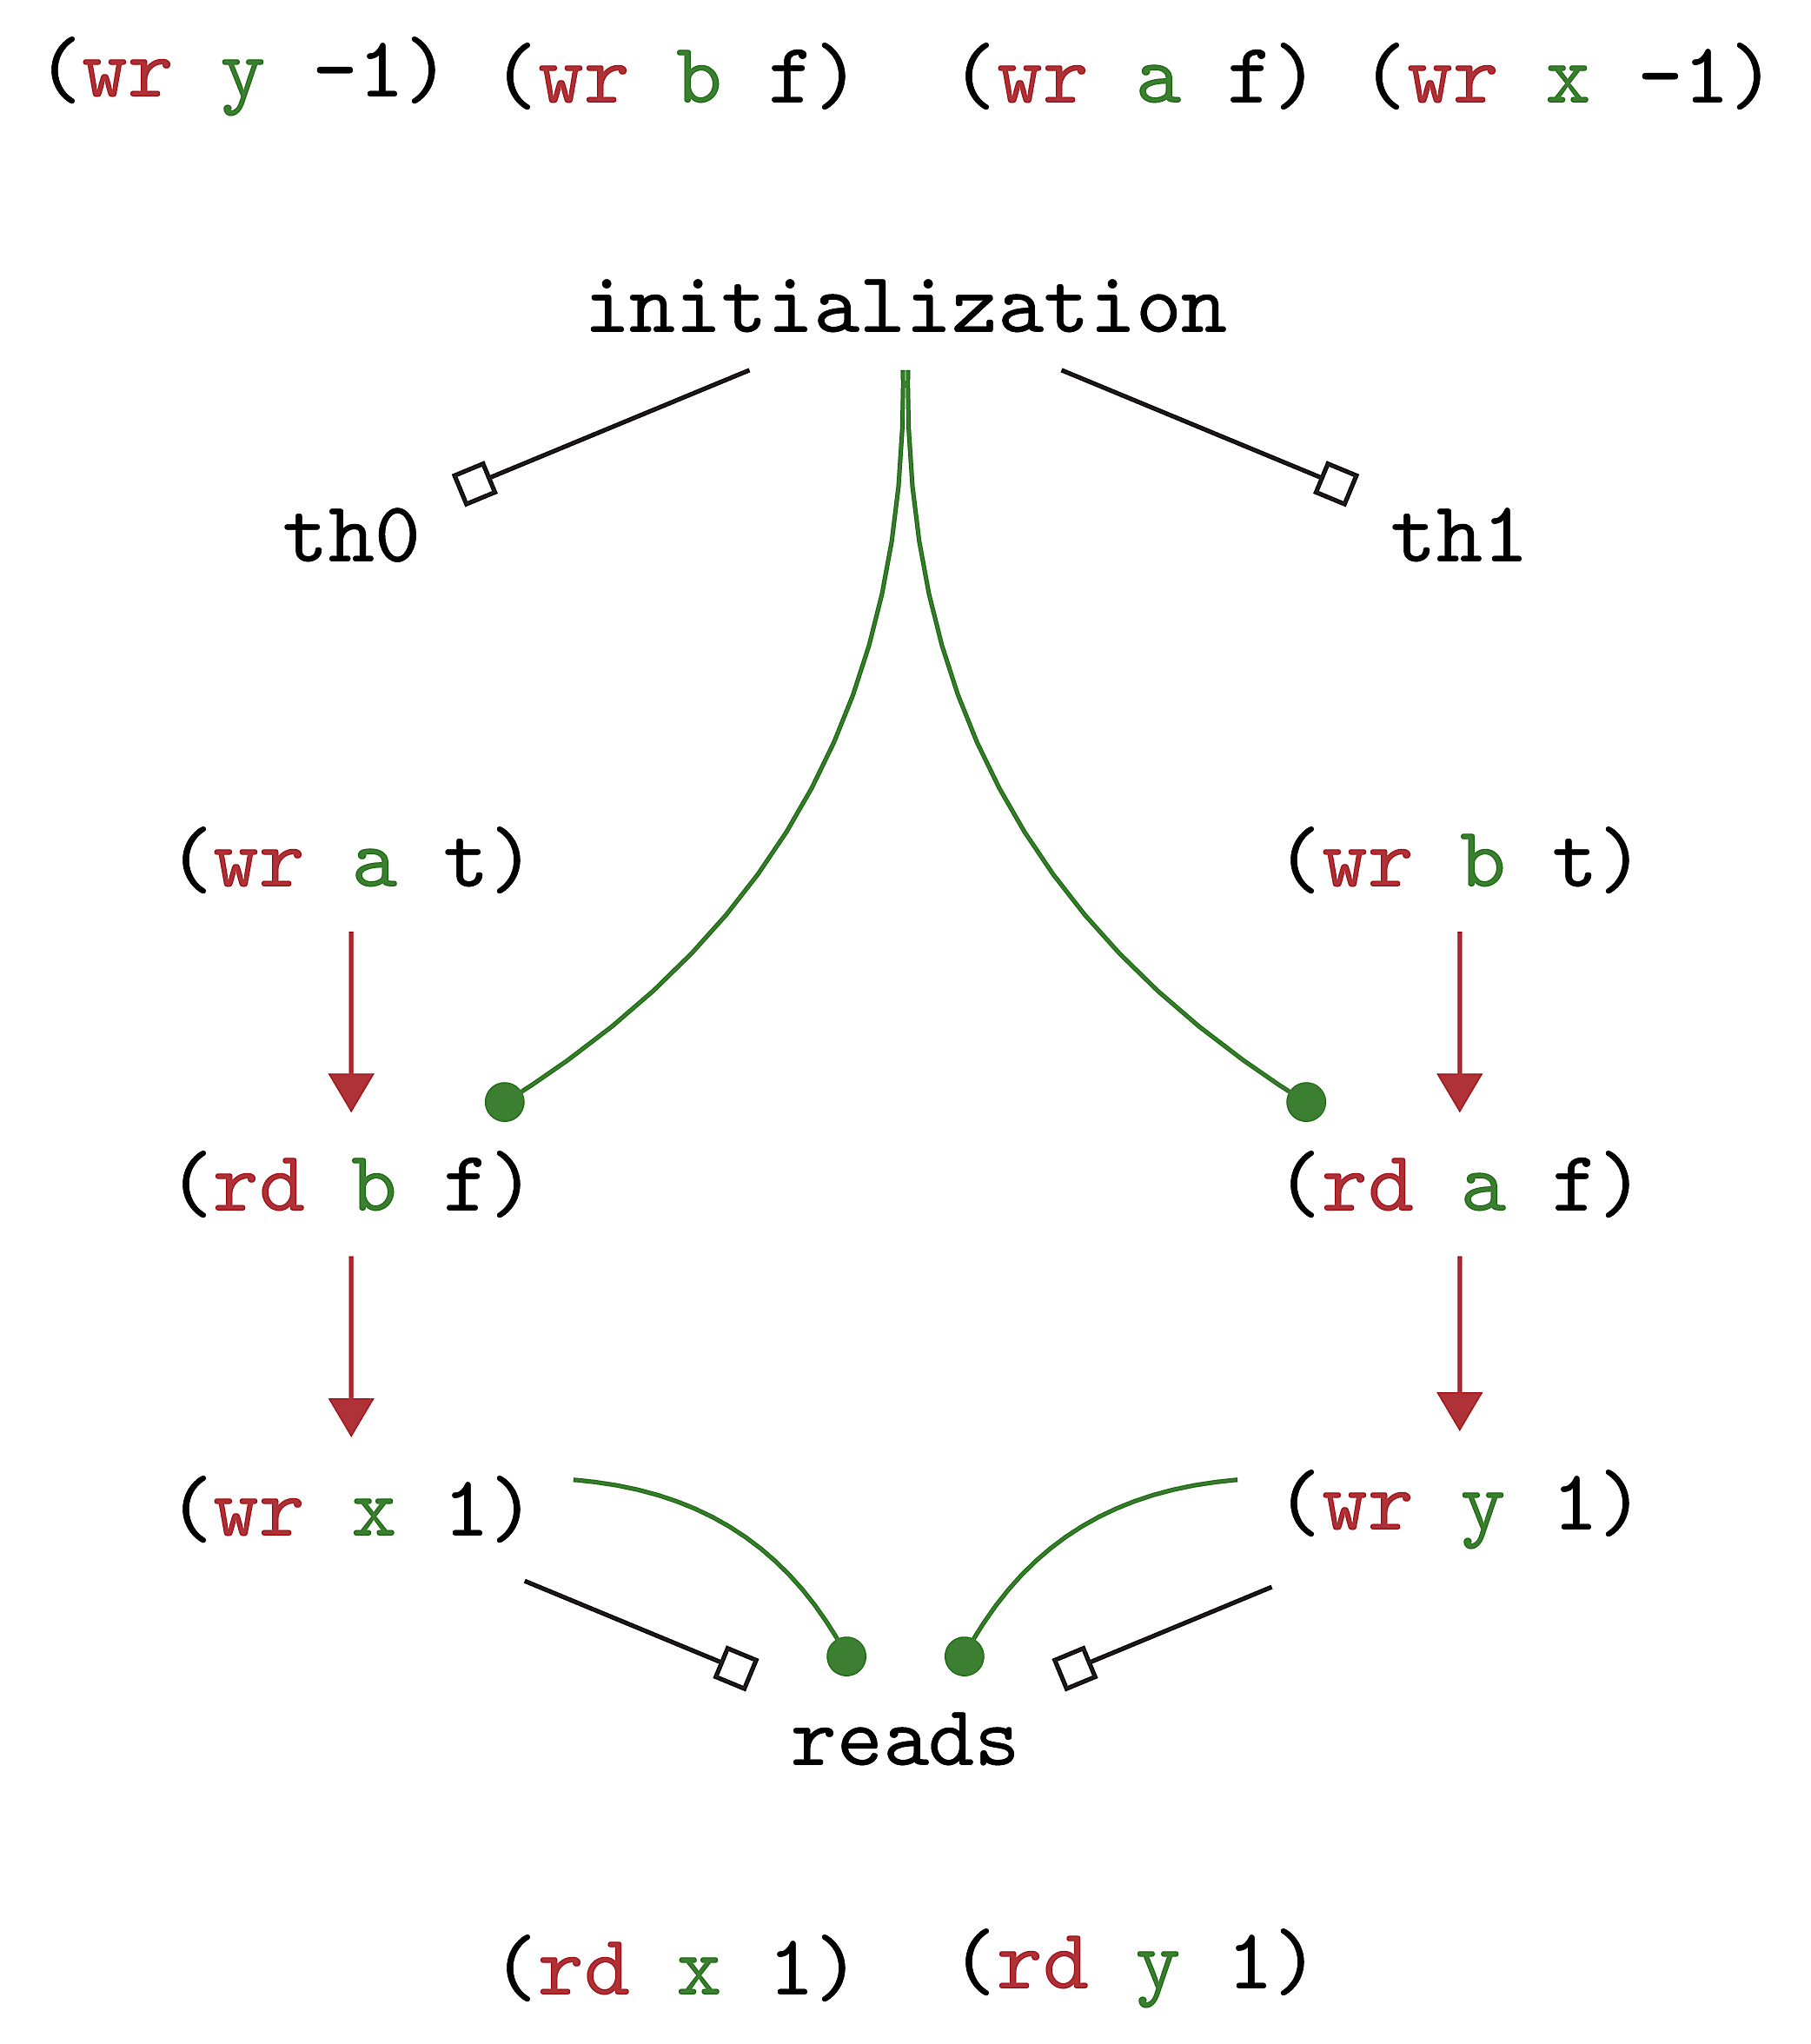
\includegraphics[height=0.9\textheight]{fig/trace5-11-5.jpg}

\end{frame}

% myths

\begin{frame}
    \frametitle{Myth: my program is compiled per the spec}

    The spec is described on an abstract machine. The runtime only \emph{emulates} it.

    \pause

    As long as no one can call your bluff, you're good.

    \pause

    Swap statements? Remove entire blocks? As long as no one, \emph{anywhere},
    can differentiate the resulting effects, go ahead.

    \pause

    Pain: students seem to \emph{love} thinking about compiler reorderings. To
    the JMM spec, they don't exist. Students refuse to accept this.

\end{frame}

\begin{frame}[fragile]
    \frametitle{"Locks" as a mental model}

\begin{lstlisting}
var x: Int = 0
var y: Int = 0
\end{lstlisting}

\begin{multicols}{2}
\begin{lstlisting}
// t0
synchronized {x = 1}
synchronized {y = 1}
\end{lstlisting}

\columnbreak

\begin{lstlisting}
// t1
val a = y
val b = x
println((a, b))
\end{lstlisting}
\end{multicols}

\centering
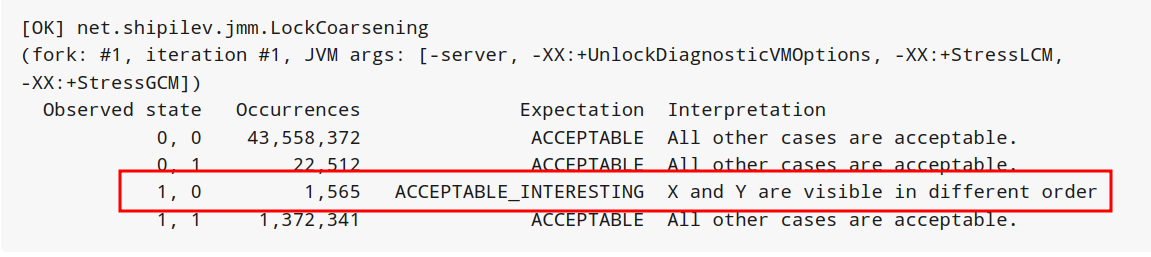
\includegraphics[height=8em]{fig/xyswap.png}

\end{frame}

\begin{frame}[fragile]
    \frametitle{"Commit to memory" as a mental model}

    \begin{lstlisting}
var x: Int = 0
var y: Int = 0
    \end{lstlisting}
    
    \begin{multicols}{4}
        \begin{lstlisting}
// t0
x = 1
        \end{lstlisting}
        \columnbreak
        \begin{lstlisting}
// t1
y = 1
        \end{lstlisting}
        \columnbreak
        \begin{lstlisting}
// t2
val a = x
val b = y
(a, b)
        \end{lstlisting}
        \columnbreak
        \begin{lstlisting}
// t3
val b = y
val a = x
(a, b)
        \end{lstlisting}        
    \end{multicols}

    \pause
    Possible to read \lstinline|t2: (x = 1, y = 0), t3: (x = 0, y = 1)|!

    \pause
    \emph{Pain: lack of "multi-copy atomicity".} If many threads are reading a
    variable, their history of those reads do not need to be consistent in
    general. Hardware-dependent!

\end{frame}

\begin{frame}[fragile]
    \frametitle{"Fences" as a mental model}

\begin{lstlisting}
@volatile var greatBarrierReef: Int = 0
var x: Int = 0
var y: Int = 0
\end{lstlisting}

\begin{multicols}{2}
\begin{lstlisting}
// t0
x = 1
y = 1
greatBarrierReef = 1
\end{lstlisting}

\columnbreak

\begin{lstlisting}
// t1
greatBarrierReef = 2
(x, y)
\end{lstlisting}
\end{multicols}

\pause
Surely it's not possible to read \lstinline|x = 0, y = 1|...? \pause Exactly 1 out of 1M 
\includegraphics[height=1em]{fig/kiss.png}

\end{frame}

\begin{frame}
    \frametitle{"Separability" as a mental model}

    \centering
    \emph{If I write \textbf{my} code well, I'm good!}

    \begin{itemize}
        \item Separate memory locations you touch
        \item Carefully analyze critical sections
    \end{itemize}

    \pause

    \vspace{2em}
    
\includegraphics[width=0.3\textwidth]{fig/smiley.jpg}

\end{frame}

\begin{frame}[fragile]
    \frametitle{"Separability" as a mental model}

    
\begin{lstlisting}
var x: Int = 0 // your territory
var y: Int = 0 // your nailbiting neighbour's
\end{lstlisting}
            \begin{multicols}{2}
                \begin{lstlisting}
// t0
y = 1
x = 1
val a = y
val c = x
                \end{lstlisting}
        
                \columnbreak
        
                \begin{lstlisting}
// t1
x = 2
y = 2
val b = y
val d = x
                \end{lstlisting}
            \end{multicols}

\phantom{a}

\end{frame}

\begin{frame}[fragile]
    \frametitle{"Separability" as a mental model}

    
\begin{lstlisting}
var x: Int = 0 // your territory
@volatile var y: Int = 0 // neighbour felt unsafe 
\end{lstlisting}
            \begin{multicols}{2}
                \begin{lstlisting}
// t0
y = 1
x = 1
val a = y
val c = x
                \end{lstlisting}
        
                \columnbreak
        
                \begin{lstlisting}
// t1
x = 2
y = 2
val b = y
val d = x
                \end{lstlisting}
            \end{multicols}

\pause
You are now implicitly attached to an abstract, and \emph{very fragile}, global
state! 

\end{frame}

% start examples ----

\begin{frame}[fragile]
    \frametitle{Not everything is an \lstinline|Int|}

    \begin{lstlisting}
var a: Long = 0L
    \end{lstlisting}
    \begin{multicols}{2}
        \begin{lstlisting}
// t0
a = 70000000000L
        \end{lstlisting}

        \columnbreak

        \begin{lstlisting}
// t1
a = 80000000000L
println(a)
        \end{lstlisting}
    \end{multicols}

    Outputs? \pause 0? \pause 70000000000L?\pause ~80000000000L?\pause  ~78589934592L \dots?

    \pause \emph{Other technical baggage: access atomicity v memory ordering and the burden of volatility}

\end{frame}

\begin{frame}[fragile]
    \frametitle{Horror Circus: sync on strings}

\begin{multicols}{2}
\begin{lstlisting}
// t0
"Lock".synchronized {
    x = x + 1
} 
\end{lstlisting}
\columnbreak

\begin{lstlisting}
// t1
"Lock".synchronized {
    x = x + 1
} 
\end{lstlisting}
\end{multicols}

\end{frame}

\begin{frame}
    More horrific examples on: 

    \fullcite{encounters}

    \begin{center}
        
\includegraphics[height=10em]{fig/closeencounters.png}
    \end{center}

\end{frame}

\begin{frame}
    \frametitle{Print everything!}

    \pause
    \setlength{\columnsep}{-20ex}
    \begin{multicols}{2}
        
\includegraphics[width=0.6\columnwidth]{fig/sniper.jpg}\pause

        \columnbreak

        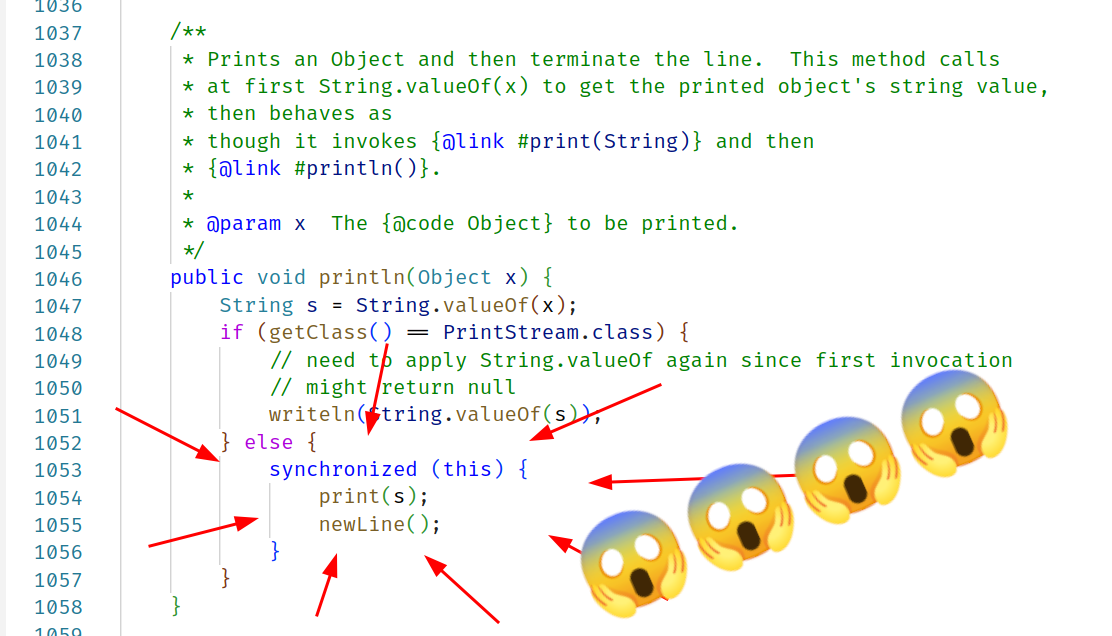
\includegraphics[width=1.2\columnwidth]{fig/java_print.png}
    \end{multicols}

\end{frame}

\begin{frame}
    \frametitle{Conclusions}

    \begin{itemize}
        \item Not much
        \item Take what you can
        \item Don't write concurrent code (yourself)
    \end{itemize}

\end{frame}

\begin{frame}

    \printbibliography

\end{frame}

\end{document}
